\documentclass[conference]{IEEEtran}
\IEEEoverridecommandlockouts
% The preceding line is only needed to identify funding in the first footnote. If that is unneeded, please comment it out.
\usepackage{cite}
\usepackage{amsmath,amssymb,amsfonts}
\usepackage{algorithmic}
\usepackage{graphicx}
\usepackage{textcomp}
\usepackage{xcolor}
\def\BibTeX{{\rm B\kern-.05em{\sc i\kern-.025em b}\kern-.08em
    T\kern-.1667em\lower.7ex\hbox{E}\kern-.125emX}}
\begin{document}

\newcommand{\authoremail}[2]{%
  \IEEEauthorblockN{#1}
  \IEEEauthorblockA{\textit{University of Alabama at Birmingham} \\ #2}
}

\title{GPT (to be changed)}

\author{\authoremail{Michael Gathara}{mikegtr@uab.edu}
\and
\authoremail{Yang (Jason) Liu}{yliu0602@uab.edu}
\and
\authoremail{Vaishak Menon}{vmenon19@uab.edu}
\and
\authoremail{Elizabeth Molen}{emolen@uab.edu}
\and
\authoremail{Trenton Davis}{trentd@uab.edu}
\and
\authoremail{Akshar Patel}{akshar2020@uab.edu}
}

\maketitle

\begin{abstract}
Large language models (LLMs) are a subset of artificial intelligence (AI)
models that have the ability to intake, understand, and generate human 
readable text. Since their inception, these models have found rapid success and widespread adoption in a vast range of industries and 
use cases including software engineering, healthcare, insurance, 
and supply-chain management. The most powerful LLMs are often built on 
an architectural framework called a transformer which calculates importance of different parts of the input and weighs the relationship between 
them in order to produce more coherent and relevant outputs. A specific type of LLM- generative pretrained 
transformers (GPTs)- stand out as one of the most used and adopted models as
they are tuned to be highly effective at understanding conversational 
context and generating coherent and relevant text. Built on top of the transformer architecture, GPTs are often more
finely tuned to perform specific tasks after
first being trained on a large corupus of less specific textual data- hence the pre-trained portion of the name. While the transformer has remained the 
core of these models, many different optimizations have been proposed and 
implemented over the past several years including flash attention, blank, and blank. In this work, we implement a scratch-built GPT equipped with some 
of these optimizations, train it on several different datasets, and then test 
it on several tasks and analyze some of the features of the model. 
\end{abstract}


\section{Introduction}
In recent years, artificial intelligence (AI) models have been gaining popularity in both personal use 
as well as in industry adoption. Among these models, none seem to have risen to such a high level of 
popular adoption as large language models (LLMs) which are AI models that can intake, understand, and generate
human-readable text \cite{brown2020languagemodelsfewshotlearners}. Usage of these has gained traction in a broad 
range of industries including 
research, healthcare, supply-chain, and software engineering 
\cite {liang2024mappingincreasingusellms} \cite{ZHANG2025102883} \cite{urlana2024llmsindustriallensdeciphering}. 
The most powerful LLMs are often built on 
an architectural framework called a transformer which calculates importance of different parts of the input and weighs 
the relationship between them in order to produce more coherent and relevant outputs.
In their seminal 2017 paper, Vaswani et al. introduced the 
transformer architecture and set the stage for the many iterations of LLMs that 
have come in the years since \cite{vaswani2023attentionneed}. This original paper focused on the core attention 
component of the transformer which calculates the interactions between different
input tokens and uses this contextual knowledge to more dynamically generate 
relevant output text. While a transformative architecture, the core attention mechanism does suffer from 
a few key drawbacks that have motivated the need for some important optimizations in the years since. 
Because it calculates interactions between every input token pair, the attention mechanism suffers from 
a quadratic time and memory complexity leading to some amnesia inducing context length limitations. Additionally, 
models immediately following the transformer architecture follow a single uniform application of the attention 
mechanism at their different layers. This lack of heterogenity and depth didn't allow the models to 
fully capture the nuanced and dynamic interactions between the input tokens.

Generative pre-trained transformers (GPTs) are a specific instantiation of LLMs that use the transformer architecture as a backbone. 
GPTs are engineered to be highly effective at generating relevant text and at performing 
conversationally oriented tasks by first pre-training them on a huge corpus of text and then fine tuning
them for their specific tasks- a process that was introduced by Radford et al. \cite{radford2018improving}. Following 
that initial introduction, GPTs utilizing magnitudes more parameters began to be explored- consistently
increasing their usefulness in conversational tasks. Specifically, post-training capacity of the 
models to learn and respond to instructions deliverd to them as inputs was detailed by Brown et al. in their 
2020 paper introducing GPT-3 \cite{brown2020languagemodelsfewshotlearners}. 
While making significant bounds in model performance and practical usefulness, these architectures still 
suffered from the same core limitations of the original transformer setup that they are built on top of. 

In the present work, we implement a from-scratch trained GPT architecture but we also explore some of the 
optimizations that have been introduced to address the aformentioned limitations of the transformer architecture. 
Two of the core optimizations that we utilize are flash-attention and multi-head latent attention. Flash attention  addresses
the issue of quadratic memory complexity in the original attention mechanism- an issue that significantly slows down 
the computation as expensive GPU memory transfers abound with full attention scores being computed and scored. 
Flash attention focuses on making the attention mechanism input/output (IO) aware and splits the computations 
into tiles that can fit on a GPUs on-chip memory and eschew temporally costly IO operations \cite{dao2022flashattentionfastmemoryefficientexact}.
 In our setup, we use flash attention and see significant improvements in our model training time as well as inference.


\section{Methods}
We present a transformer-based language model that employs a novel attention mechanism called Multi-headed Latent Attention (MLA). This section details the architecture of our model and the training methodology.
\subsection{Model Architecture}
Our model follows the general transformer architecture~\cite{vaswani2017attention} with several key modifications. The model consists of 12 transformer layers, each containing a multiheaded latent attention module and a feed-forward network. We use an embedding dimension of 768 and 12 attention heads throughout the model. The context window is limited to 512 tokens.
The input token sequence is first embedded using a token embedding layer and combined with learned positional embeddings:
\begin{equation}
h_0 = W_e \cdot x + W_p
\end{equation}
\noindent where $W_e \in \mathbb{R}^{V \times d}$ is the token embedding matrix for vocabulary size $V$ and embedding dimension $d$, and $W_p \in \mathbb{R}^{n \times d}$ is the positional embedding matrix for a maximum sequence length $n$.
\subsubsection{Multi-headed Latent Attention (MLA)}
\textcolor{red}{Jason do you want to write about MLA here?}
\subsubsection{Feed-Forward Networks}
After the attention layer, each transformer block contains a feed-forward network using SwiGLU activation~\cite{shazeer2020glu}, which has been shown to outperform ReLU in language models. The feed-forward network is defined as:
\begin{align}
\text{Swish}(xW_1) \otimes (xW_2) \
\text{FFN}(x) = \text{SwiGLU}(x)W_3
\end{align}
\noindent where $W_1, W_2 \in \mathbb{R}^{d \times 4d}$ and $W_3 \in \mathbb{R}^{4d \times d}$ are learned parameter matrices, $\text{Swish}(x) = x \cdot \sigma(x)$ is the swish activation function, and $\otimes$ represents element-wise multiplication.
Each attention and feed-forward sublayer is wrapped with a residual connection and layer normalization:
\begin{align}
  h'_i &= \mathrm{LN}(h_i) \\
  h_{i+\frac12} &= h_i + \mathrm{MLA}(h'_i) \\
  h''_{i+\frac12} &= \mathrm{LN}(h_{i+\frac12}) \\
  h_{i+1} &= h_{i+\frac12} + \mathrm{FFN}(h''_{i+\frac12})
\end{align}
\noindent where $\text{LN}$ denotes layer normalization.
\subsubsection{Tokenization}
We train a custom Byte-Pair Encoding (BPE) tokenizer~\cite{sennrich2016neural} on the Wikitext-103 corpus with a vocabulary size of 32,000. The tokenizer includes special tokens \texttt{[PAD]}, \texttt{[UNK]}, \texttt{[CLS]}, \texttt{[SEP]}, \texttt{[MASK]}, \texttt{[BOS]}, and \texttt{[EOS]}. We use whitespace pre-tokenization and set a minimum token frequency of 2 to filter out rare tokens.
\subsection{Training}
\subsubsection{Dataset}
We train our model on the Wikitext-103 corpus~\cite{merity2016pointer}, a collection of good quality Wikipedia articles containing approximately xxx million tokens. Prior to tokenization, we apply a text cleaning procedure to remove markup elements and normalize whitespace. The cleaned text is then tokenized and chunked into sequences of 512 tokens for training.
\subsubsection{Training Process}
The model is trained using distributed data parallelism across multiple NVIDIA H100 GPUs. We employ mixed precision training (FP16) with gradient scaling to improve computational efficiency while maintaining numerical stability. The training process uses a batch size of 72 per GPU with gradient accumulation over 4 steps, resulting in an effective batch size of 288.
We implement model parallelism using PyTorch's DistributedDataParallel (DDP) framework. The dataset is partitioned across GPUs using a DistributedSampler to ensure each worker processes different data. The training loop includes the following steps:
\begin{enumerate}
    \item Sample a batch $(x, y)$ from the data loader
    \item Perform a forward pass with mixed precision: $\text{logits}, \text{loss} = \text{model}(x, y)$
    \item Scale the loss
    \item Perform a backward pass with gradient scaling
    \item If $i \bmod \text{accumulation_steps} = 0$:
    \begin{enumerate}
        \item Clip gradients to maximum norm 1.0
        \item Update model parameters
        \item Zero gradients
        \item Update learning rate with scheduler
    \end{enumerate}
    \item If $i \bmod \text{eval_interval} = 0$:
    \begin{enumerate}
        \item Evaluate on validation set
        \item Save checkpoint if validation loss improved
    \end{enumerate}
\end{enumerate}
\noindent This process continues for a maximum of 15,000 iterations or until convergence.
\subsubsection{Optimization}
We optimize our model using AdamW~\cite{loshchilov2018decoupled} with a weight decay of $1 \times 10^{-4}$ and beta parameters $\beta_1 = 0.9$, $\beta_2 = 0.95$. The initial learning rate is set to $1 \times 10^{-3}$.
Our learning rate schedule combines a linear warmup phase with a cosine decay phase:
\begin{equation}
\text{lr}(t) =
\begin{cases}
\text{lr}{\text{max}} \cdot \frac{t}{\text{warmup}} & \text{if } t < \text{warmup} \\
\ldots
\end{cases}
\end{equation}
\noindent where $\text{warmup} = 500$ iterations and $\text{max} = 15,000$ iterations. This schedule helps stabilize early training and gradually reduces the learning rate to achieve better convergence.
\noindent where \textit{warmup steps} eq 500 and \textit{max steps} eq 15,000. This schedule helps stabilize early training and gradually reduces the learning rate to achieve better convergence.
To prevent gradient explosion, we apply gradient clipping with a maximum norm of 1.0 before each optimizer step.
\subsubsection{Hyperparameter Tuning}
To optimize model performance, hyperparameter tuning and testing was performed on the flash attention and MLA architectures. 
Both architectures were trained for 5000 iterations on nine combinations of three transformer layer values (10, 12, and 14) and three attention head values (8, 10, and 12). 
These hyperparameters were selected for potential for noticeable impact on model performance.
All other hyperparameters remained the same during training and testing except for embedding dimensions which were adjusted to 760 (from 768) for models trained with 10 attention heads. 
This was done to account for the requirement that the number of attention heads evenly divide the embedding dimensions. A test dataset was then used to calculate average model loss and perplexity values for each of the nine hyperparamater combinations to further assess and compare model performances.
The training process for all models followed the evaluation and checkpointing methodology and testing methodology discussed in the following sections. 


\subsubsection{Evaluation and Checkpointing}
We evaluate the model on the validation set every 100 iterations by computing the average loss over multiple batches. The best model is selected based on the lowest validation loss achieved during training. Additionally, we save periodic checkpoints every 500 iterations to enable resumption of training if needed.
To monitor training progress, we log key metrics including training loss, validation loss, learning rate, and throughput (tokens processed per second) using TensorBoard. After training, we generate sample text from the best checkpoint to qualitatively assess the model's capabilities.
\subsection{Testing}
For the testing of our model, we used two different primary metrics: loss and perplexity. The loss function that we utilized both in our model training as 
well as in the testing is the standard cross-entropy loss i.e. 
\begin{equation}
\mathcal{L}_{\text{CE}}
  \;=\;
  -\frac{1}{N}\sum_{i=1}^{N}\sum_{c=1}^{C}
  y_{i,c}\;\log p_{i,c},
\end{equation}
where $y_{i,c} \in \{0,1\}$ is the one-hot reference label for example $i$ and class $c$, and $p_{i,c}$ is the model's predicted probability for that class.
And the perplexity is defined as:
\begin{equation}
\operatorname{PPL}
  \;=\;
  \exp\!\bigl(
      -\tfrac{1}{T}\sum_{t=1}^{T} \log p(w_t \mid w_{<t})
    \bigr),
\end{equation}
where $p(w_t \mid w_{<t})$ is the model’s predicted probability of token $w_t$ given its history $w_{<t}$.
In addition to these two metrics, we also qualitatively evaluate the model's performance by generating sample text from 
each of the model checkpoints that we test. 


\subsection{Model Architecture}
\input{sections/architecture.tex}

\subsection{Training}
\input{sections/training.tex}

\subsection{Evaluation and Introspection}
\input{sections/eval.tex}

\section{Results}
Results from model training and testing fell into three categories: loss, and perplexity, and subjective assessment of text output quality.

\subsection{Loss and Perplexity}
Best validation model loss, average test dataset loss and test dataset perplexity were collected for all tested models (see Figures \ref{best_loss}, \ref{avg_loss}, and \ref{perplexity}).
Loss and perplexity values were noticeably higher for the flash attention architecture on all models tested.

\begin{figure}[H]
    \centering
    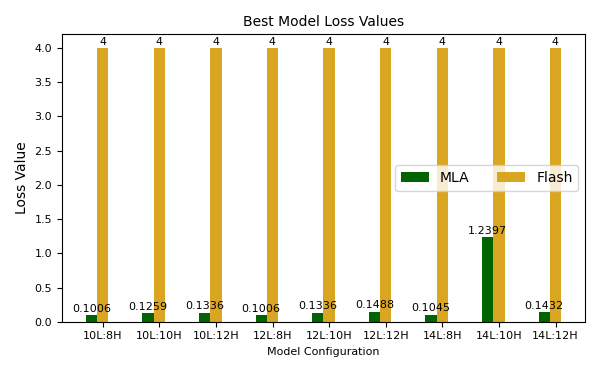
\includegraphics[width=\linewidth]{sections/images/best_loss.png}
    \caption{Best model loss for all tested models. L represents number of transformer layers. H represents number of attention heads.}
    \label{best_loss}
\end{figure}

\begin{figure}[H]
    \centering
    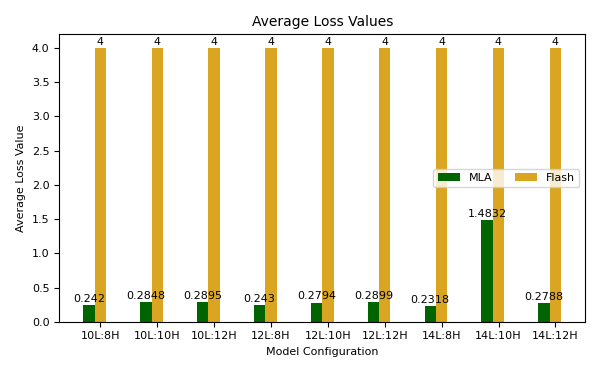
\includegraphics[width=\linewidth]{sections/images/avg_loss.png}
    \caption{Average model loss for all tested models. L represents number of transformer layers. H represents number of attention heads.}
    \label{avg_loss}
\end{figure}

\begin{figure}[H]
    \centering
    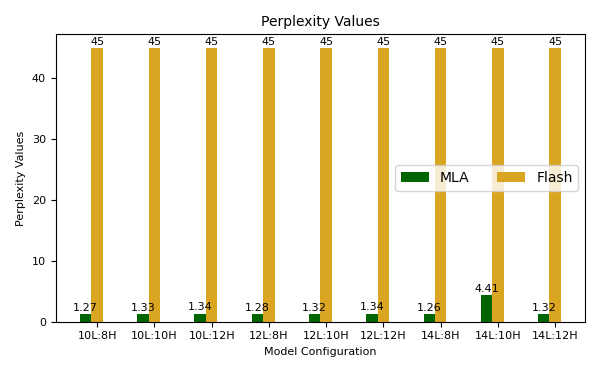
\includegraphics[width=\linewidth]{sections/images/perplexity.png}
    \caption{Perplexity loss for all tested models. L represents number of transformer layers. H represents number of attention heads.}
    \label{perplexity}
\end{figure}

\subsection{Subjective Assessment of Text Output Quality}
Text output from training and validation of each model configuration was reviewed by multiple team members. 
Several models were also provided custom prompts and output was assesed.
Taking into consideration factors such as sentence structure, text coherence, and word variability, the flash attention performed superiorly to MLA for all models tested\n.

General sentence flow and content for the flash attention model was readable and fairly coherent but generally lacked specificty and detail.  
Overall MLA models produced far less coherent text than the flash attention and contained may reptitions of a single word, which varied from model to model.
For MLA, models with higher loss and perplexity performed superiorly, suggesting a tendency for the models to overfit at the tested parameters.

\section{Discussion}

\subsection{Results Analysis}
Average loss, best model loss, and perplexity values were higher for the flash attention architecture than for the MLA architecture configuration models as a whole. However, the 
flash attention still produced superior textual output.   
This was likely due to several factors, such as:
\subsubsection{MLA Implementation and Hyperparameter Selection}



\subsubsection{Something Else}

% Ending subsubsection

Interestingly, one MLA hyperparamter configuration model (14 layers, 10 transformer heads) had much higher average loss and perplexity values than other configurations. 
While higher loss and perplexity can often be associated with worse performance, this model model also performed better under the subjective textual analysis.  
This supports that the models were overfitting.

\subsection{Challenges}
The leading challenges of this project was the computational power and time required to train and test models. 
For example, with the MLA architecture, additional testing on MLA-specific hyperparameters, such as number of latent vector and dimensionality of latent 
nubmer of latent vectors and dimensionality of latent vector space.  


\subsubsection{Dataset Size}


\subsection{Future Work}
This project presents numerous opportunities for future work. 
Further research should include refining the MLA architecture and testing on additional hyperparameters to attempt to prevent the observed overfitting and repetitive words issues.
In addition, given the appearance of overfitting on the flash attention architecture, it should be tested with additional hyperparameters, as well.
Finally, results were likely 

\section{Conclusion}
{}

\break{}
\bibliographystyle{IEEEtran}
\bibliography{references} % .bib 

\end{document}
